\documentclass[11pt,oneside]{article}
\usepackage[utf8]{inputenc}
\usepackage[american]{babel}
\usepackage{setspace}
\usepackage{microtype}
\usepackage{mathpazo} % Palantino font
\usepackage{mdframed}
\usepackage{pgfplots}
\usepackage{minted}
  \setminted{fontsize=\small}
  \setminted{breaklines}
  \usemintedstyle{bw}
  \BeforeBeginEnvironment{minted}{\vspace{6pt}\begin{mdframed}[topline=false,rightline=false,bottomline=false,linecolor=black,linewidth=2pt]}
  \AfterEndEnvironment{minted}{\end{mdframed}}
\usepackage{xcolor}
\usepackage{graphicx}
\newcommand\dd[1]{\colorbox{gray!30}{\texttt{#1}}}
\usepackage{hyperref}
  \hypersetup{colorlinks=true,allcolors=blue!40!black}
\pagestyle{empty}
\setstretch{1.1}
\setlength{\topskip}{6pt}
\setlength{\parindent}{0pt} % indent first line
\setlength{\parskip}{6pt} % before par

\title{
\includegraphics[scale=0.05]{logo.png}\\Zold: a Light-Weight Crypto Currency}
\author{Yegor Bugayenko\\\texttt{yegor@zold.io}}

\begin{document}
\raggedbottom

\maketitle
\begin{abstract}
In the last few years digital currencies successfully demonstrated
their ability to become an alternative financial instrument in many
different markets. Most of the technologies available at the moment are
based on the principles of Blockchain architecture, including the
dominating currencies like Bitcoin and Etherium. Despite its
popularity, Blockchain is not the only possible solution. Zold is
an \emph{experimental} alternative that enables distributed transactions between
anonymous users. It borrows the ``proof of work'' principle from Bitcoin,
and suggests a different architecture for digital wallets maintenance.
\end{abstract}

\colorbox{yellow}{It's a draft! Don't show it to anyone yet.}

\section{Motivation}

Bitcoin, the first decentralized digital currency, was released in
January 2009. Since then a number of similar Blockchain-based products have been
created, including Etherium, Litecoin, and others. \colorbox{yellow}{links} There were other solutions,
not based on Blockchain, including IOTA, and others. \colorbox{yellow}{links}

Zold is also a decentralized digital currency that maintains its transactions
in an unpredicable amount of zero-trust server nodes, trying to guarantee
data consistency. However, the architecture of Zold is not based on Blockchain
principles. The development of Zold was motivated by the desire to overcome
a few obvious disadvantages of existing solutions.

First, the speed of transaction processing is rather low. \colorbox{yellow}{proof?}

Second, mining commissions are high. \colorbox{yellow}{proof?}

Third, the technology is too complex. \colorbox{yellow}{proof?}

Zold was created as an attempt to resolve these mentioned problems
of existing digital currencies.

%%%%%%%%%%%%%%%%%%%%%%%%%%%%%%%%%%%%%%%%%%%%%%%%%%%%%%%%%%%%%%%%%%%%%%%%%%%%%%%%%%%%%%%%%%%%%%%%%%%
%%%%%%%%%%%%%%%%%%%%%%%%%%%%%%%%%%%%%%%%%%%%%%%%%%%%%%%%%%%%%%%%%%%%%%%%%%%%%%%%%%%%%%%%%%%%%%%%%%%
%%%%%%%%%%%%%%%%%%%%%%%%%%%%%%%%%%%%%%%%%%%%%%%%%%%%%%%%%%%%%%%%%%%%%%%%%%%%%%%%%%%%%%%%%%%%%%%%%%%
\section{Principles}

\textbf{Open Source}.
Zold is a command line tool. Its entire code base is open source
and hosted at the GitHub \href{https://github.com/yegor256/zold}{yegor256/zold}
repository.

\textbf{No Trust}.
The network of communicating nodes maintains wallets of users.
Anyone can add a node to the network.
It is assumed that any node may contain corrupted data, either by mistake or intentionally.

\textbf{Proof of work}.
Each node, in order to earn trust, must invest its CPU power
and find hash suffixes, performing certain expensive and meaningless calculations.

\textbf{No General Ledger}.
There is no central ledger, each wallet has its own personal ledger.
All transactions in each ledger are confirmed by
\href{https://en.wikipedia.org/wiki/RSA_(cryptosystem)}{RSA signatures}
of their owners.

\textbf{Capacity}.
One currency unit is called ZLD.
One ZLD by convention equals to $2^{24}$ \emph{zents} (16,777,216).
All amounts are stored as signed 64-bit integers.
Thus, the technical capacity of the currency is 549,755,813,888 ZLD (half a trillion).

\textbf{Root Wallet}.
Zold is a pre-mined currency.
The only way to get ZLD is to receive it from someone else.
The root wallet belongs to the issuer and may have a negative balance,
which can grow according to a pre-defined restrictive formula.
All other wallets may only have positive balances.

\colorbox{yellow}{Let's compare each of these principles with other currencies and highlight similarities.}

%%%%%%%%%%%%%%%%%%%%%%%%%%%%%%%%%%%%%%%%%%%%%%%%%%%%%%%%%%%%%%%%%%%%%%%%%%%%%%%%%%%%%%%%%%%%%%%%%%%
%%%%%%%%%%%%%%%%%%%%%%%%%%%%%%%%%%%%%%%%%%%%%%%%%%%%%%%%%%%%%%%%%%%%%%%%%%%%%%%%%%%%%%%%%%%%%%%%%%%
%%%%%%%%%%%%%%%%%%%%%%%%%%%%%%%%%%%%%%%%%%%%%%%%%%%%%%%%%%%%%%%%%%%%%%%%%%%%%%%%%%%%%%%%%%%%%%%%%%%
\section{Proof of Work}

The system consists of nodes (server machines), which maintain the data.
In order to guarantee data consistency among all distributed nodes
there has to be an algorithm of data segregation.
Corrupted data must be detected earlier and filtered out as quickly as possible.
Bitcoin introduced such an algorithm and called it \emph{proof of work}.
\colorbox{yellow}{link}

Its fundamental principle is that each block of data must have a special
number attached to it, known as \emph{nonce}, which is rather difficult to calculate,
because it requires a lot of CPU power. It is assumed that at any moment
of time the majority of nodes in the network invest their CPU power into
calculating the nonces for the data that is not corrupted. If and when for any reason
some data gets corrupted, the amount of CPU power a part of the network
decides to invest into its nonces calculation would be smaller than what
the other part of the network invests into legal data. The latter part
will quickly dominate the former and the nodes with corrupted data will
be ostracized and eventually ignored.
\colorbox{yellow}{let's make sure this text is correct and add a link}

Zold has borrowed this principle, although modified it. It also requires
its nodes to invest their CPU power into meaninless and repetative
calculations just to help us identify which part of the network they belong to:
corrupted or not. Each Zold node has to calculate its \emph{trust score},
which is as big as much CPU power the node has invested into its calculation.

Similar to Bitcoin nonces we repetatively calculate cryptographic hashes,
looking for consecutive zeros inside them. First, in order to calculate a score,
a node makes the \emph{prefix}, which consists of four parts,
separated by spaces:

\begin{enumerate}
\item The current timestamp in UTC, in \href{https://en.wikipedia.org/wiki/ISO_8601}{ISO 8601},
\item The host name or IP address, e.g. \dd{b2.zold.io},
\item The \href{https://en.wikipedia.org/wiki/Port_(computer_networking)}{TCP port} number,
\item The invoice.
\end{enumerate}

For example, the prefix may look like this:

\begin{minted}{text}
2018-05-17T03:50:59Z b2.zold.io 4096 THdonv1E@0000000000000000
\end{minted}

Then, the node attempts to append any arbitrary text, which has to match
\dd{/[a-zA-Z0-9]+/} regular expression, to the end of the prefix and calculates
\href{https://en.wikipedia.org/wiki/SHA-2}{SHA-256 hash} (\colorbox{yellow}{why not SHA-3?})
of the text in the hexadecimal format. For example, this would be the prefix
with the attached \dd{117b1f} suffix:

\begin{minted}{text}
2018-05-17T03:50:59Z b2.zold.io 4096 THdonv1E@0000000000000000 117b1f
\end{minted}

The hash of this text will be:

\begin{minted}{text}
670baa704726fe2c837c5ca764202adca5ab12c9b90c94d9fb1b8d629000000
\end{minted}

The node attempts to try different sufficies until one of them produces
a hash that ends with a few tailing zeroes. The one above ends
with six zeroes
(it took three minutes to find it on 2.3GHz Intel Core i7):

When the first suffix is found, the score is 1. Then, to
increase the score by one, the next suffix has to be found, which
can be added to the first 64 characters of the previous hash
in order to obtain a new hash with trailing zeros, for example:

\begin{minted}{text}
2018-05-17T03:50:59Z b2.zold.io 4096 THdonv1E@0000000000000000 117b1f 1546e35
\end{minted}

Produces:

\begin{minted}{text}
99dcd18e4bd03004e1205437866b5b68035cc8985240ae52cbd37640a000000
\end{minted}

And so on.

The score is valid only when the starting time point is earlier than
the current time, but not earlier than 24 hours ago. The strength of the score
is the amount of the trailing zeros in the hash. In the example above the
strength is six.

%%%%%%%%%%%%%%%%%%%%%%%%%%%%%%%%%%%%%%%%%%%%%%%%%%%%%%%%%%%%%%%%%%%%%%%%%%%%%%%%%%%%%%%%%%%%%%%%%%%
%%%%%%%%%%%%%%%%%%%%%%%%%%%%%%%%%%%%%%%%%%%%%%%%%%%%%%%%%%%%%%%%%%%%%%%%%%%%%%%%%%%%%%%%%%%%%%%%%%%
%%%%%%%%%%%%%%%%%%%%%%%%%%%%%%%%%%%%%%%%%%%%%%%%%%%%%%%%%%%%%%%%%%%%%%%%%%%%%%%%%%%%%%%%%%%%%%%%%%%
\section{Wallets}

There is no central ledger in Zold, like many other digital currencies.
Instead, each user has their own \emph{wallets} (any number of them) with their own ledgers inside.
Each wallet is an ASCII-text file with the name equal to the wallet ID.
For example, the wallet in the file \dd{12345678abcdef} may include:

\begin{minted}{text}
zold
0.6.4
12345678abcdef
AAAAB3NzaC1yc2EAAAADAQABAAABAQCuLuVr4Tl2sXoN5Zb7b6SKMPrVjLxb...

003a;2017-07-19T21:24:51Z;ffffffff9c0ccccd;Ui0wpLu7;98bb82c81735c4ee;For services;SKMPrVj...
003b;2017-07-19T21:25:07Z;ffffffffffa72367;xksQuJa9;98bb82c81735c4ee;For food;QCuLuVr4...
0f34;2017-07-19T21:29:11Z;0000000000647388;kkIZo09s;18bb82dd1735b6e9;-;
003c;2017-07-19T22:18:43Z;ffffffffff884733;pplIe28s;38ab8fc8e735c4fc;For programming;2sXoN5...
\end{minted}

Lines are separated by either CR or CRLF.
There is a header and a ledger, separated by an empty line.
The header includes four lines:

\begin{enumerate}
  \item Network name, \dd{[a-z]\{4,16\}};
  \item Software version, \dd{[0-9]+(\.[0-9]+)\{1,2\}} (\href{https://semver.org/}{semantic versioning});
  \item Wallet ID, a 64-bit unsigned integer in hexadecimal format;
  \item Public \href{https://en.wikipedia.org/wiki/RSA_(cryptosystem)}{RSA}
    key of the wallet owner, in \href{https://en.wikipedia.org/wiki/Base64}{Base64}.
\end{enumerate}

The ledger includes transactions, one per line. Each transaction line
contains fields separated by a semi-colon:

\begin{enumerate}
  \item \dd{id}: Transaction ID, an unsigned 16-bit integer, 4-symbols hex;
  \item \dd{time}: date and time, in \href{https://en.wikipedia.org/wiki/ISO_8601}{ISO 8601} format, 20 symbols;
  \item \dd{amount}: Zents, a signed 64-bit integer, 16-symbols hex;
  \item \dd{prefix}: Payment prefix, 8-32 symbols;
  \item \dd{bnf}: Wallet ID of the beneficiary, 16-symbols hex;
  \item \dd{details}: Arbitrary text, matching \dd{/[a-zA-Z0-9 -.]\{1,512\}/};
  \item \dd{signature}: \href{https://en.wikipedia.org/wiki/RSA_(cryptosystem)}{RSA} signature,
    684 symbols in \href{https://en.wikipedia.org/wiki/Base64}{Base64}.
\end{enumerate}

Transactions with positive amount don't have signatures.
Their IDs point to ID fields of corresponding beneficiaries' wallets.

The combination \dd{id}+\dd{bnf}
must be unique in the entire wallet.

The \href{https://en.wikipedia.org/wiki/RSA_(cryptosystem)}{RSA}
signature is calculated using the private key of the
wallet and the following fields of transaction, separated by spaces:
\dd{bnf}, \dd{id}, \dd{time}, \dd{amount}, \dd{prefix}, \dd{bnf}, \dd{details}.

For example, this text may be used as a signing input:

\begin{minted}{text}
12345678abcdef 003a 2017-07-19T21:24:51Z ffffffff9c0ccccd Ui0wpLu7 98bb82c81735c4ee For services
\end{minted}

Each transaction takes 1284 symbols at most.

The order of transactions is not important, as long as their final balance is positive.

%%%%%%%%%%%%%%%%%%%%%%%%%%%%%%%%%%%%%%%%%%%%%%%%%%%%%%%%%%%%%%%%%%%%%%%%%%%%%%%%%%%%%%%%%%%%%%%%%%%
%%%%%%%%%%%%%%%%%%%%%%%%%%%%%%%%%%%%%%%%%%%%%%%%%%%%%%%%%%%%%%%%%%%%%%%%%%%%%%%%%%%%%%%%%%%%%%%%%%%
%%%%%%%%%%%%%%%%%%%%%%%%%%%%%%%%%%%%%%%%%%%%%%%%%%%%%%%%%%%%%%%%%%%%%%%%%%%%%%%%%%%%%%%%%%%%%%%%%%%
\section{Mining Formula}

The only way to get ZLD is to receive it from the \emph{root} wallet \dd{0000000000000000}.
This wallet is the only one that may have a negative ballance.
However, to prevent an uncontrolled emission of ZLD, the balance
of this wallet must satisfy the formula:

$$x = \frac{2048}{h};\quad z = 2^{63 - x}.$$

Here $h$ is the age of the root wallet in hours and $z$ is the maximum
amount of zents it can issue at that moment. The first
six years will look like this:

\vspace{\parskip}\begin{center}\begin{tabular}{lrr}
\hline
Year & ZLD & Share \\
\hline
1st & 32m & 0.01\% \\
2nd & 4b & 0.77\% \\
3rd & 21b & 4\%\\
4th & 48b & 9\% \\
5th & 78b & 14\% \\
6th & 108b & 20\% \\
\hline
\end{tabular}\end{center}

On a large perspective of 25 years total emission of ZLD will look
like this:

\vspace{\parskip}\begin{center}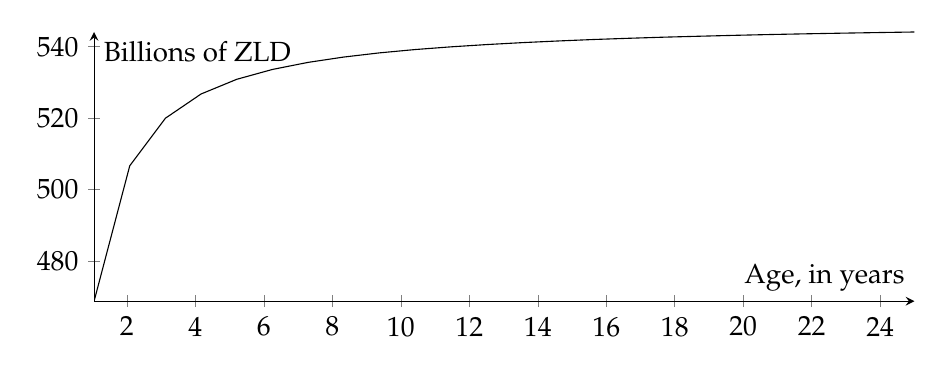
\begin{tikzpicture}
\begin{axis}[
  axis lines=middle,
  width=12cm,height=5cm,
  xlabel={Age, in years},
  ylabel={Billions of ZLD},
]
\addplot[domain=-0:25, samples=25]{2^(39-2048/(x*24*365)) / 1000000000};
\end{axis}
\end{tikzpicture}\end{center}

The limitation is hardwired in Zold software and can't be eliminated.

%%%%%%%%%%%%%%%%%%%%%%%%%%%%%%%%%%%%%%%%%%%%%%%%%%%%%%%%%%%%%%%%%%%%%%%%%%%%%%%%%%%%%%%%%%%%%%%%%%%
%%%%%%%%%%%%%%%%%%%%%%%%%%%%%%%%%%%%%%%%%%%%%%%%%%%%%%%%%%%%%%%%%%%%%%%%%%%%%%%%%%%%%%%%%%%%%%%%%%%
%%%%%%%%%%%%%%%%%%%%%%%%%%%%%%%%%%%%%%%%%%%%%%%%%%%%%%%%%%%%%%%%%%%%%%%%%%%%%%%%%%%%%%%%%%%%%%%%%%%
\section{Taxes}

Each wallet must have to pay \emph{taxes} in order to be promoted by nodes.
The maximum amount of tax debt a node can tolerate is 1 ZLD. This means
that if the debt is smaller, all nodes must promote the wallet to their
remote nodes. If the debt is bigger, a node will reject the wallet,
which will make it impossible to make any new payments from it.

The amount of taxes to be paid is calculated by the following formula:

$$X = A \times F \times T.$$

$A$ is the total age of the wallet,
which is calculated as the difference in hours between the current time
and the time of the oldest transaction in the wallet.
$T$ is the total number of transactions in the wallet.
$F$ is the fee per transaction/hour, which is equal to 7.48 zents
(a one-year-old wallet with 4096 transactions must pay approximately 16 ZLD taxes annually).

In order to pay taxes the owner of the wallet has to select any remote
node from the network, which has a score of 16 or more. Then, it has to
take the invoice from the score, request the node to lock the score
for a minute, and send the payment of 1 ZLD or less
to that node. The score with exactly 16 suffixes
has to be placed into the details of the transaction,
prefixed by \dd{TAXES }.

The most active remote node will be selected as tax receiver.
It's up to the payer which node to select.

All tax payments inside a wallet must have unique scores.
Duplicate tax payments are ignored.

%%%%%%%%%%%%%%%%%%%%%%%%%%%%%%%%%%%%%%%%%%%%%%%%%%%%%%%%%%%%%%%%%%%%%%%%%%%%%%%%%%%%%%%%%%%%%%%%%%%
%%%%%%%%%%%%%%%%%%%%%%%%%%%%%%%%%%%%%%%%%%%%%%%%%%%%%%%%%%%%%%%%%%%%%%%%%%%%%%%%%%%%%%%%%%%%%%%%%%%
%%%%%%%%%%%%%%%%%%%%%%%%%%%%%%%%%%%%%%%%%%%%%%%%%%%%%%%%%%%%%%%%%%%%%%%%%%%%%%%%%%%%%%%%%%%%%%%%%%%
\section{Remote Nodes}

Each node maintains a list of \emph{remote nodes} (their host names and TCP port numbers),
their scores and their availability information. When the node is just installed,
the list contains a limited amount of pre-defined addresses. The list is
updated both by user request and automatically in order to give priority
to high-score nodes and the nodes with the highest availability.
Moreover, the node adds new elements to the list retrieving them from all
available remote nodes.

The built-in mechanism pays attention to the following factors of
remote node \emph{quality} (in order of importance):

  * Visibility: the payer has to know the node,
  * Availability: the amount of errors seen recently,
  * Knowledgeability: the amount of nodes this node is aware of,
  * Activity: the frequency of push requests the node originates,
  * Score: the one reported during the most recent handshake.

%%%%%%%%%%%%%%%%%%%%%%%%%%%%%%%%%%%%%%%%%%%%%%%%%%%%%%%%%%%%%%%%%%%%%%%%%%%%%%%%%%%%%%%%%%%%%%%%%%%
%%%%%%%%%%%%%%%%%%%%%%%%%%%%%%%%%%%%%%%%%%%%%%%%%%%%%%%%%%%%%%%%%%%%%%%%%%%%%%%%%%%%%%%%%%%%%%%%%%%
%%%%%%%%%%%%%%%%%%%%%%%%%%%%%%%%%%%%%%%%%%%%%%%%%%%%%%%%%%%%%%%%%%%%%%%%%%%%%%%%%%%%%%%%%%%%%%%%%%%
\section{Fetch, Merge, and Propagate}

First, to see a wallet, it has to be \emph{fetched} from a number of remote
nodes. The nodes may provide different versions of the same wallet, either
because some data is corrupted or because modifications were made to the same
wallet from different parts of the network. Each version retrieved from the
network is stored in a local \emph{copy} and gets a score assigned to it.
The score of the local copy is a summary of all scores of the nodes that
provided that copy. Let's say, there are 17 nodes in the network and they
provided three different copies of the wallet:

\begin{minted}{text}
copy-1: 78,090 bytes, 11 servers, 177 score
copy-2: 56,113 bytes, 4 servers, 69 score
copy-3: 97,132 bytes, 2 servers, 37 score
\end{minted}

The fetch operation ends at this point. The next step is to \emph{merge}
all three copies into the local one, if it exists. The algorithm of merging
is the following.

First, the copy of the wallet we are merging into, is added to the list,
with the score zero:

\begin{minted}{text}
copy-0: 55,991 bytes, 0 servers, 0 score
copy-1: 78,090 bytes, 11 servers, 177 score
copy-2: 56,113 bytes, 4 servers, 69 score
copy-3: 97,132 bytes, 2 servers, 37 score
\end{minted}

Then, the copy with the highest score is assumed to be the correct one,
which is the \dd{copy-1} in this example.

Then, all other copies, in the order of their scores, are merged into the
correct one, transaction by transaction, applied the following rules
consequently:

\begin{enumerate}
\item If the transaction already exists, it's ignored;
\item If the transaction is negative (spending money) and its ID is lower than
the maximum ID in the ledger, it gets ignored as a fraudulent one (``double spending'');
\item If the transaction makes the balance of the wallet negative, it is ignored;
\item If the transaction is positive and its signature is not valid, it is ignored;
\item If the transaction is negative and it's absent in the paying wallet
(which is fetched and merged first), it's ignored;
\item Otherwise, it gets added to the end of the ledger.
\end{enumerate}

When merge is done, the modifications get \emph{propagated} to other wallets
available locally. Each transaction that has a negative amount is
copied to the ledger of their receiving wallets (with a reversed sign),
if it doesn't yet exist there.

%%%%%%%%%%%%%%%%%%%%%%%%%%%%%%%%%%%%%%%%%%%%%%%%%%%%%%%%%%%%%%%%%%%%%%%%%%%%%%%%%%%%%%%%%%%%%%%%%%%
%%%%%%%%%%%%%%%%%%%%%%%%%%%%%%%%%%%%%%%%%%%%%%%%%%%%%%%%%%%%%%%%%%%%%%%%%%%%%%%%%%%%%%%%%%%%%%%%%%%
%%%%%%%%%%%%%%%%%%%%%%%%%%%%%%%%%%%%%%%%%%%%%%%%%%%%%%%%%%%%%%%%%%%%%%%%%%%%%%%%%%%%%%%%%%%%%%%%%%%
\section{Pay and Push}

To send money from one wallet to another, the owner of the sending wallet
has to add a negative transaction to it and sign it with the private RSA key.

At any moment of time any node may decide to push a wallet to another node.
The receiving node accepts it, merges with the local version, and keeps locally.
Then, it \emph{promotes} the wallet to all known remote nodes.

%%%%%%%%%%%%%%%%%%%%%%%%%%%%%%%%%%%%%%%%%%%%%%%%%%%%%%%%%%%%%%%%%%%%%%%%%%%%%%%%%%%%%%%%%%%%%%%%%%%
%%%%%%%%%%%%%%%%%%%%%%%%%%%%%%%%%%%%%%%%%%%%%%%%%%%%%%%%%%%%%%%%%%%%%%%%%%%%%%%%%%%%%%%%%%%%%%%%%%%
%%%%%%%%%%%%%%%%%%%%%%%%%%%%%%%%%%%%%%%%%%%%%%%%%%%%%%%%%%%%%%%%%%%%%%%%%%%%%%%%%%%%%%%%%%%%%%%%%%%
\section{RESTful API}

There is a limited set of RESTful API entry points in each node.
Each response has \dd{Content-Type},
\dd{Content-Length}, and \dd{X-Zold-Version}
HTTP headers.

\dd{GET /} is a home page of a node that returns JSON/200 response with the
information about the node, for example (other details may be added in
further versions):

\begin{minted}{json}
{
  "version": "0.6.1",
  "score": {
    "value": 3,
    "host": "b2.zold.io",
    "port": 4096,
    "invoice": "THdonv1E@0000000000000000",
    "suffixes": [ "4f9c38", "49c074", "24829a" ],
    "strength": 6
  }
}
\end{minted}

\dd{GET /remotes} returns the list of remote nodes known by the node,
in JSON/200:

\begin{minted}{json}
{
  "version": "0.6.1",
  "all": [
    { "host": "b2.zold.io", "port": 4096 },
    { "host": "b1.zold.io", "port": 80 }
  ]
}\end{minted}

\dd{GET /wallet/<ID>} returns the content of the wallet, in JSON/200:

\begin{minted}{json}
{
  "version": "0.6.1",
  "body": "..."
}\end{minted}

If the wallet is not found, a
\href{https://www.w3.org/Protocols/rfc2616/rfc2616-sec10.html#sec10.4.5}{404}
HTTP response is returned.

If the client provided the MD5 hash of the wallet content in the
\href{https://www.w3.org/Protocols/rfc2616/rfc2616-sec14.html#sec14.26}{\dd{If-None-Match}}
HTTP header and it matches with the hash of the
content the node contains, a
\href{https://www.w3.org/Protocols/rfc2616/rfc2616-sec10.html#sec10.3.5}{304} HTTP response is returned.

\dd{PUT /wallet/<ID>} pushes the content of the wallet to the node. The
node responds either with
\href{https://www.w3.org/Protocols/rfc2616/rfc2616-sec10.html#sec10.2.3}{202} (if accepted),
\href{https://www.w3.org/Protocols/rfc2616/rfc2616-sec10.html#sec10.4.1}{400} (if the data is corrupted),
\href{https://www.w3.org/Protocols/rfc2616/rfc2616-sec10.html#sec10.4.3}{402} (if taxes are not paid),
or
\href{https://www.w3.org/Protocols/rfc2616/rfc2616-sec10.html#sec10.3.5}{304}
(if the content is the same as the one the node already has).

%%%%%%%%%%%%%%%%%%%%%%%%%%%%%%%%%%%%%%%%%%%%%%%%%%%%%%%%%%%%%%%%%%%%%%%%%%%%%%%%%%%%%%%%%%%%%%%%%%%
%%%%%%%%%%%%%%%%%%%%%%%%%%%%%%%%%%%%%%%%%%%%%%%%%%%%%%%%%%%%%%%%%%%%%%%%%%%%%%%%%%%%%%%%%%%%%%%%%%%
%%%%%%%%%%%%%%%%%%%%%%%%%%%%%%%%%%%%%%%%%%%%%%%%%%%%%%%%%%%%%%%%%%%%%%%%%%%%%%%%%%%%%%%%%%%%%%%%%%%
\section{Incentives}

It is obvious that anonymous users will participate in Zold and maintain
their nodes only if they have enough financial motivation to do that. Simply
put, their expenses must be lower than the income they are getting in
form of taxes. This Section analyzes the most obvious questions users
may have, regarding their motivation.

\subsection{To Stay Online}

What is the reason for a node to stay online and spend its CPU power
and network traffic? Each node is insterested in doing that because it
hopes that wallet owners will pay taxes to its invoices. The software
automatically decides which node to pay taxes to and the selection is
made by the availability criteria. The node which is the most available
and visible will get the majority of tax payments.

\subsection{To Accept Wallets}

Why a node would accept push requests and spend its storage space
on the wallets coming in? If the node doesn't accept a push request,
its availability rating decreases and other nodes will stop paying
taxes to it.

\subsection{To Advertise Other Nodes}

What is the incentive to advertise other remote nodes via the \dd{/remotes} RESTful
entry point and why can't a node always return an empty list, expecting its clients
to always pay taxes to it? The software automatically prioritizes remote
nodes by the amount of remote nodes it promotes. The longer the list a node
returns, the higher its chance to be at the top of the list.

\subsection{To Promote Wallets}

What is the incentive to promote wallets to remote nodes, spending network
traffic for this operation?

\colorbox{yellow}{We need more here}

%%%%%%%%%%%%%%%%%%%%%%%%%%%%%%%%%%%%%%%%%%%%%%%%%%%%%%%%%%%%%%%%%%%%%%%%%%%%%%%%%%%%%%%%%%%%%%%%%%%
%%%%%%%%%%%%%%%%%%%%%%%%%%%%%%%%%%%%%%%%%%%%%%%%%%%%%%%%%%%%%%%%%%%%%%%%%%%%%%%%%%%%%%%%%%%%%%%%%%%
%%%%%%%%%%%%%%%%%%%%%%%%%%%%%%%%%%%%%%%%%%%%%%%%%%%%%%%%%%%%%%%%%%%%%%%%%%%%%%%%%%%%%%%%%%%%%%%%%%%
\section{Threats}

It is obvious that a distributed system that consists of anonymous nodes
even theorecially can't be 100\% safe, reliable, secure and trustworthy.
Zold is not an exception. However, it's designed in an honest attempt
to mitigate all critical threats and make the system ``reliable enough.''
This Section summarizes the most import of those threads and explains
how Zold responds to them.

\subsection{Double Spending}

It is possible to submit the same spending transaction to the same wallet
and then push it to two different nodes in different parts of the network.
They won't know about each other and will propagate those spending
transactions to other wallets. Both two owners of those money receiving
wallets will think that their money arrived, while only one of them is
a legit receiver, the other transaction is fraudulent.

This will happen, but very soon one part of the network will dominate the other
one, and one of the transactions will be rejected from the wallet, after
a number of merge operations in all nodes of the network. The receiver of the
money must be careful and always to the full fetch (from as many

\subsection{Fraudulent Tax Refunds}

Some nodes may resell their scores to their affiliated tax payers, and they
refund them some amount of taxes back. This will be profitable both for
the tax payers, since they will pay less taxes, and for the node owners,
since they will receive the payments anyway.

This scenario is indeed possible, but we assume that since tax payments are
supposed to be made in small increments and automatically, the majority of
clients won't be interested in this fraudulent scheme.

\colorbox{yellow}{We need more here}

\end{document}
